\section{A Shrinking Circle Problem}
\label{sec:applied_limit_problem}

\subsection*{Recommended Tutorials:}
\begin{itemize}[noitemsep]
	\item \nameref{chp:equation_solvers}, pg. \pageref{chp:equation_solvers}
	\item \nameref{chp:limits}, pg. \pageref{chp:limits}
\end{itemize}

\subsection*{Introduction:}

Limits may seem trivial when you first learn them, but they are fundamental building blocks in calculus. They are used to explain terms like ``infinitesimally small'' and ``infinitely large''. It may be interesting to know that they can also be used in applied problems. This activity will explore a geometry problem and will solve it using limits, instead of an elementary geometric approach.

Figure \ref{fig:applied_limit} below shows two circles:
\begin{itemize}
	\item $C_1$, centred at the point $(1,0)$ with radius $1$ and equation \[(x-1)^2+y^2=1.\]
	\item $C_2$, centred at the origin with radius $r$ and equation \[x^2+y^2=r^2.\]
\end{itemize}

\begin{figure}[h]
\centering
\label{fig:applied_limit}
\caption{What happens to the point $R$ as the radius of the thicker circle $C_2$ shrinks?}
\pgfplotsset{compat=1.5.1}
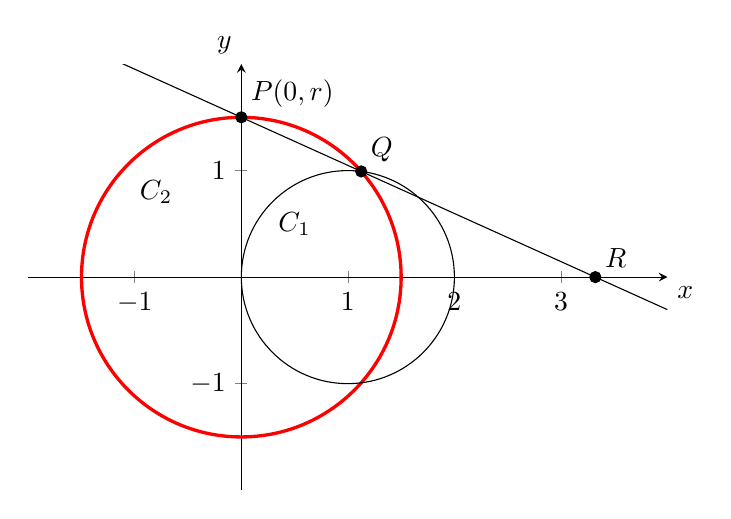
\begin{tikzpicture}[shift={(0,0)}]
	\begin{axis}[
	width=0.8\linewidth,
	axis lines=middle,
	xlabel={$x$},
	ylabel={$y$},
	xlabel style={below right},
	ylabel style={above left},
	xmin=-2, xmax=4, xtick={-1,0,1,2,3},
	ymin=-2, ymax=2, ytick={-1,0,1},
    axis equal image
	]
	\addplot[domain=-2:4] {1.500000000-.4514162296*x};
	\addplot[mark=*] coordinates {(0,1.5)} node [above right] {$P (0,r)$};
	\addplot[mark=*] coordinates {(1.125000000,0.9921567417)} node [above right] {$Q$};
	\addplot[mark=*] coordinates {(3.322875656,0)} node [above right] {$R$};
	\draw(axis cs:0,0) [very thick, red] circle[radius=1.5];
	\draw(axis cs:-0.8,0.8) node {$C_2$};
	\draw(axis cs:1,0) circle[radius=1];
	\draw(axis cs:0.5,0.5) node {$C_1$};
	\end{axis}
\end{tikzpicture}
\end{figure}

If we define $P$ as the point $(0,r)$ at the top of the circle $C_2$, and $Q$ as the upper point of intersection of the two circles, then we can construct the line $PQ$ and see that it crosses the $x$-axis. Let $R$ be the $x$-intercept of the line $PQ$.

\marginnote{Note that neither $P$ nor $Q$ is fixed as the radius of $C_2$ shrinks.}
Now, begin to shrink the radius of circle $C_2$; that is, let $r\rightarrow 0^{+}$. What happens to the point $R$ as $C_2$ shrinks?

\subsection*{Exercises:}

\begin{enumerate}
	\item Assign names to the equations of both circles, such as \texttt{C1} and \texttt{C2}.
    \item Find the point of intersection of $C_1$ and $C_2$ in quadrant I. This is the point $Q$. The coordinates of $Q$ should be expressions of $r$.
    \marginnote[-1cm]{You can find the point of intersection with a single \texttt{solve()} command, but you may need to include the optional parameter \texttt{explicit=true} to avoid the \textit{RootOf()} output.}\index{solving equations!removing \texttt{RootOf()}}
	\item We now have two points on the line, $P$ and $Q$, so we can construct the equation of this line. For parts (a) and (b), let $P = (0,r)$ be $(x_1,y_1)$ and let $Q$ (the point you found in exercise 2) be $(x_2,y_2)$.
	\begin{enumerate}
	\item Find the slope of the line $PQ$ using the slope equation \[ m = \frac{y_2 - y_1}{x_2 - x_1}. \]\index{lines!slope}
	\item Define the equation of the line $PQ$ using the slope from part (a) and the point-slope equation of a line	\[ y - y_0 = m (x - x_0). \]\index{lines!point-slope form}
	\end{enumerate}
	\marginnote{Remember that $R$ is the $x$-intercept of the line $PQ$, so its $y$-coordinate is $0$. The $x$-coordinate can be found using the \texttt{subs()}\index{subs}  and \texttt{solve()} \index{solving equations!solve} commands.}
	\item Using the equation of the line you just found, find the coordinates of $R$. 
	\item Now what happens as $r \to 0^+$?\index{limit}
	\marginnote{Use the \texttt{limit()} command as $r$ approaches $0$ from the right.}
\end{enumerate}

%\subsection*{Notes:}
%\begin{itemize}
  %  \item   Use 15 decimal places to find your answers, when applicable.

%\end{itemize}